\documentclass[12pt,xcolor=dvipsnames]{beamer}
\usetheme{CambridgeUS}
\usecolortheme{whale}
\setbeamercolor{block title}{use=structure,fg=white,bg=blue!75!black}  
\setbeamercolor{block body}{use=structure,fg=black,bg=blue!5!white}
\setbeamercolor{frametitle}{bg=Blue}

\usepackage{hyperref}   
\usepackage{url}
\hypersetup{urlcolor=red}

\renewcommand{\bibname}{References}
\setbeamertemplate{bibliography item}{[\theenumiv]}

\usepackage{multicol}
\usepackage{verbatim} 
\usepackage{graphics}
\usepackage{graphicx}


%Basic Information
\title{Motivation of the edX InSight Project}
\author{Arinjoy Basak, Dewang Palav, Sagar Agarwal, Ashwani Pandey, Apoorva Agarwal}
\date{\today}

%--------------------------------------------------------------------------------------
%               TITLE PAGE (Slide 1)
%--------------------------------------------------------------------------------------
\begin{document}
\begin{frame}
\titlepage
\end{frame}
%--------------------------------------------------------------------------------------


%--------------------------------------------------------------------------------------
%               Outline
%--------------------------------------------------------------------------------------
%\begin{frame}
%\frametitle{Outline}
%\begin{multicols}{2}
%\tableofcontents[hideallsubsections]
%\end{multicols}
%\end{frame}

%--------------------------------------------------------------------------------------
%               Slide 1: Topic 1
%--------------------------------------------------------------------------------------
\section{What our project is on}
\begin{frame}[t]
\frametitle{What is edX InSight?}

\begin{itemize}
\item InSight is a BI (Business Intelligence) platform that was built by edX for the purpose of communicating
the details of the courses, and analytical data concerning the student activity on the various courses to
the administrators and course instructors.\\

\item The primary aim of this platform is not only to monitor the
student performances and validation of the choices made in designing the course, but also allows the
designers to re-think the choices, and improve the course in its different aspects for creating a better
experience for the students.
\end{itemize}


%For bulleted points use the following:\\
%\begin{itemize}
% \item write point 1
% \item write poin 2
%\end{itemize}

%For numbered list use the following:\\
%\begin{enumerate}
% \item write point 1
% \item write point 2
%\end{enumerate}

\end{frame}
%--------------------------------------------------------------------------------------
%               Slide 2
%--------------------------------------------------------------------------------------
\section{What our project is on}
\begin{frame}[t]
\frametitle{What is edX InSight?}

\begin{itemize}

\item Insight is essentially a Django application that allows instructors and administrators to know about
their students with respect to.

\begin{itemize}
\item course activity
\item demographic distributions
\item location based distributions, and 
\item educational qualifications
\end{itemize}

\item The unstructured data in the form of events
are stored in Amazon S3 as JSON objects, while the processed data is then stored in MySQL. Insight
uses MySQL 5.1 for its purpose. The data is then transferred to Insights via a REST API.

\end{itemize}
\end{frame}

%--------------------------------------------------------------------------------------
%               Slide 3:
%--------------------------------------------------------------------------------------
\section{What our project is on}
\begin{frame}[t]
\frametitle{What our project is}

\begin{center}
\textit{\large "Knowledge is power"}
\end{center}

\begin{flushright}
-Francis Bacon  
\end{flushright}

\hspace{20pt} The project aims to extract maximum usable data from the huge amount of logs running into terabytes per day, and providing a concise outlook to the educators using edX platform. Using the available technologies, we want to create a workable product which presents the data in a form easy to analyse. \\

\end{frame}

%--------------------------------------------------------------------------------------
%               Slide 3: contd.
%--------------------------------------------------------------------------------------
\section{What our project is on}
\begin{frame}[t]
\frametitle{What our project is}

\begin{itemize}

\item Our main project tasks are to study the edX InSight system and contribute towards its development and final integration
with the IITBombayX MOOC Platform.

\item In particular, our aim will be to extend and implement the edX InSight services so that it appropriately suits to the 
Indian education environment.

\end{itemize}
\end{frame}

%--------------------------------------------------------------------------------------
%               Slide 4
%--------------------------------------------------------------------------------------
\section{Motivation of the edX InSight Project}
\begin{frame}[t]
\frametitle{Why do we need InSight?}

\begin{itemize}
\item The study by Ma, Han, Yang and Chen analysed the the impact of an instructor on a student’s engagement in an online learning environment, by building an interaction activity model for the teaching and learning process.

\item It was showed that learning data analytics could be used
to capture authentic, timely and objective evidence regarding online learning behaviour, with a focus
towards college level online learning environments.

\item The course was the unit of analysis, not the student.

\end{itemize}
\end{frame}
%--------------------------------------------------------------------------------------
%               Slide 5
%--------------------------------------------------------------------------------------
\section{Motivation of the edX InSight Project}
\begin{frame}[t]
\frametitle{Why do we need InSight?}

edX Insight provides access to various graphs, metrics and reports for analysing the student behaviour and activity in different aspects, such as :

\begin{itemize}

\item Course Enrollment data : daily student enrollment chart, enrollment metric, and enrollment over time metrics.

\item Engagement Data : weekly engagement charts, content engagement breakdown report.
\item Demographic Data : analytics on age bands and educational backgrounds.
\item Location/Geographic Data : enrollment geography.
\item Data on graded and ungraded contents : Find points of difficulty, and attempts to solve the problems.

\end{itemize}
\end{frame}

%--------------------------------------------------------------------------------------
%               Slide 6
%--------------------------------------------------------------------------------------
\section{Motivation of the edX InSight Project}
\begin{frame}[t]
\frametitle{Project Application Ideas to present}

The following ideas were developed by the respective members of the group

\begin{itemize}
\item Arinjoy Basak
\item Dewang Palav
\item Sagar Agarwal
\item Ashwani Pandey
\item Apoorva Agarwal
\end{itemize}
\end{frame}

%--------------------------------------------------------------------------------------
%               Slide 7
%--------------------------------------------------------------------------------------
\section{Motivation of the edX InSight Project}
\begin{frame}[t]
\frametitle{Project application idea 1 (Arinjoy Basak)}

\begin{itemize}
\item Analyse the student learning behaviour and activities through the pauses in the lecture videos.
\item The locations of the pauses could be collected as events, and metrics could be developed and appropraite visualizations made to notify or warn the instructors about the difficulty faced by students in particular parts of materials.
\item This could then be met by appropriate measures on the teacher's end, such as

\begin{itemize}
\item Adding more explanatory material
\item Release of an expansion video
\item More quizzes ad practice exercises.
\end{itemize}

\end{itemize}
\end{frame}

%--------------------------------------------------------------------------------------
%               Slide 8
%--------------------------------------------------------------------------------------
\section{Motivation of the edX InSight Project}
\begin{frame}[t]
\frametitle{Project application idea 1 (Arinjoy Basak)}
\hfill
\hfill
\begin{itemize}
\item API exists for such tracking, and we can have a possible flow such as the following:
\hfill
\begin{center}
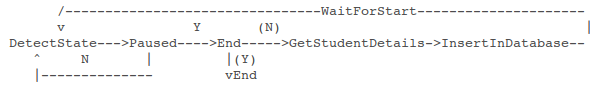
\includegraphics[height=1.8cm]{Diag1.png}\\ % Insert your image it this way
\end{center}

\end{itemize}

\end{frame}

%--------------------------------------------------------------------------------------
%               Slide 9
%--------------------------------------------------------------------------------------
\section{Motivation of the edX InSight Project}
\begin{frame}[t]
\frametitle{Project application idea 2 (Arinjoy Basak)}

\begin{itemize}
\item Create dashboard system for students based on their own course activity and performance
\item Allow the students to understand whether they are either falling behind the others on their progress, at par with the other students, or ahead of the other students in learning
\item This could be implemented as a mobile application too, refreshed with the analysed data and visualizations after a certain time period.
\item Inspired by Erik Duval's speech at TEDxUHowest
\end{itemize}
\end{frame}

%--------------------------------------------------------------------------------------
%               Slide 10
%--------------------------------------------------------------------------------------
\section{Motivation of the edX InSight Project}
\begin{frame}[t]
\frametitle{Project application idea 3 (Arinjoy Basak)}

\begin{itemize}
\item The communication and interaction between the students could be collected
\hfill
\item We can then use this data to visualize the communication and interaction between the students, to find he students/student groups who are in close communication, and those who aren't in close communication and are slightly outside this conglomerate, residing on the edges.
\item Inspired by Erik Duval's speech at TEDxUHowest
\end{itemize}
\end{frame}

%--------------------------------------------------------------------------------------
%               Slide 11
%--------------------------------------------------------------------------------------
\section{Motivation of the edX InSight Project}
\begin{frame}[t]
\frametitle{Project application idea 4 (Arinjoy Basak)}

\begin{itemize}
\item A spectral band image system for determining the student's performance

\begin{itemize}
\item ---) Because people understand images better than text or data! (:D)
\end{itemize}

\item The spectrum would have different colours for different areas (examinations, lessons, mood of students, activity overall)
\item Intensity of the colours depicts performance.
\item The degree of transitions between the individual regions determines the balance of the activities.

\end{itemize}
\end{frame}

%--------------------------------------------------------------------------------------
%               Slide 12
%--------------------------------------------------------------------------------------
\section{Motivation of the edX InSight Project}
\begin{frame}[t]
\frametitle{Project application idea 5 (Arinjoy Basak)}

\begin{itemize}
\item For each pair of students chosen at a time, show a graphical measure to determine interaction among any two students chosen at a time.
\item For example, a colour spectrum with the degree of transition showing the amount of interaction between the students (may even extend to student and teacher/instructor)
\item Can be used for determining homogeneity in student population and points of disturbances (less interaction, ineffective activity, behind others in progress, and so on).

\end{itemize}
\end{frame}

%--------------------------------------------------------------------------------------
%               Slide 13
%--------------------------------------------------------------------------------------
\section{Motivation of the edX InSight Project}
\begin{frame}[t]
\frametitle{Project application ideas (Dewang Palav)}

Applications:
\begin{itemize}
 \item The consistency graph of a student's time of attempting a test gives an insight into the level of seriousness of a student towards a course.\\
 \item A certain extent of dynamic behaviour can be implemented by real time time-per-question statistics.\\
 \item The courses can be personalized to a greater extent by the instructor with the data about the student at hand.\\
\end{itemize}
\end{frame}

%--------------------------------------------------------------------------------------
%               Slide 14
%--------------------------------------------------------------------------------------
\section{Motivation of the edX InSight Project}
\begin{frame}[t]
\frametitle{Project application ideas (Sagar Agarwal)}

Applications:
\begin{itemize}
\item Analysis of time required and performance on particular test can give information about the understanding level of students and the difficulty level of test.
\item It can also give information about difficulty level of course and hence instructor can enhance course content.

\end{itemize}
\end{frame}

%--------------------------------------------------------------------------------------
%               Slide 15
%--------------------------------------------------------------------------------------
\section{Motivation of the edX InSight Project}
\begin{frame}[t]
\frametitle{Project application ideas (Ashwani Pandey)}

Applications:
\begin{itemize}
\item Many students hesitate in asking questions or discussing their doubts.
\item In a classroom scenario, this will help the teachers see these visual analytics, and help such studetns.
\item Ultimately, this will make sure that no one is left behind in a classroom that has students with different abilities.

\end{itemize}

When provided with incentives, students will show increased interest, leading to increased learning.

\end{frame}

%--------------------------------------------------------------------------------------
%               Slide 18:
%--------------------------------------------------------------------------------------

\subsection{Motivation of the edX InSight Project}
\begin{frame}[t]
\frametitle{What answers can InSight provide? (Ashwani Pandey)}

\begin{itemize}

\item How much time students spent in viewing the videos ?
\item How much time student spent thinking on a particular question, and how many times did he try to attempt a difficult question before giving up ?
\item How active is a student on discussion boards ?
\item Are the answers and questions of the students being applauded in the discussion board ?
\item Is the student also spending equal amount of time with ungraded quizzes, and extra problems that are given to those who want to go a little bit further ?

\end{itemize}

The analytics for these questions will help figure out the interest shown by the students for a particular course.

\end{frame}

%--------------------------------------------------------------------------------------
%               Slide 18:
%--------------------------------------------------------------------------------------

\subsection{Motivation of the edX InSight Project}
\begin{frame}[t]
\frametitle{Project application ideas (Apoorva Agarwal)}

\begin{itemize}

\item Student Wise performance availaible to the teacher

\begin{itemize}
\item Weak Students
\item Strong Students
\end{itemize}

\item Generic Analytics of the course content availaible to the teacher.

\begin{itemize}
\item Average duration of answering a question for each student.
\item The strong and weak parts of course:

\begin{itemize}
\item Which part was most clear or unclear to the students.
\item Which part of the material needs to be upgraded or changed
\end{itemize}

\item The hardest or the easiest questions in the course.
\end{itemize}

\end{itemize}

\end{frame}
%--------------------------------------------------------------------------------------
%               Slide 16
%--------------------------------------------------------------------------------------
\section{Motivation of the edX InSight Project}
\begin{frame}[t]
\frametitle{Technologies to learn and apply}

Our motivation for this project is also to learn the use of the following software and applications, which besides being beneficial to IITBombayX, is also useful in our attempt to gain knowledge in the sphere of modern Big Data Analytics.

\begin{itemize}

\item EdX Platform: Edx is a recent MOOC platform developed by MIT University for offering of quality education to the students on  a large scale, through the web service. It has the potential to become the future of Education Technology.

\item Hadoop:Hadoop is an open-source software framework written in Java for distributed storage and distributed processing of very large data sets on computer clusters built from commodity hardware.

\end{itemize}
\end{frame}

%--------------------------------------------------------------------------------------
%               Slide 17
%--------------------------------------------------------------------------------------
\section{Motivation of the edX InSight Project}
\begin{frame}[t]
\frametitle{Technologies to learn and apply}

\begin{itemize}

\item Hive: Apache Hive is a data warehouse infrastructure built on top of Hadoop for providing data summarization, query, and analysis.

\item Python: Python is a widely used general-purpose, high-level programming language, emphasizing code readability, and  to express concepts in fewer lines of code than in C++ or Java.The language provides constructs intended to enable clear programs on both a small and large scale.

\item Django: A free and open source web application framework, written in Python, which follows the model-view-controller (MVC) architectural pattern.

\end{itemize}
\end{frame}

%--------------------------------------------------------------------------------------
%               Slide 18:
%--------------------------------------------------------------------------------------

\subsection{Motivation of the edX InSight Project}
\begin{frame}[t]
\frametitle{Conclusion}


\begin{itemize}

\item The concept of e-learning is gaining precedence. With IITBombayX, an indigenous implementation of the edX is pioneering this field. The need for a robust Insight mechanism which analyses the data generated is being felt at large.

\item The ultimate motivation is to meet this need with technology at hand and a contribution to the open source community.

\end{itemize}

\end{frame}



%--------------------------------------------------------------------------------------
%               Slide 3: Topic 2
%--------------------------------------------------------------------------------------
%\section{Topic 2}
%\begin{frame}[t]
%\frametitle{Topic 2}
%Use the following for creating a table \\
%\begin{center}
%\begin{tabular}{|c|c|c|}
% \hline
% No. & Name & Project \\
% \hline
% 1 & Firuza & Code::Blocks \\
% \hline
% 2 & Birundha & edX \\
% \hline
%\end{tabular}
%\end{center}
%\end{frame}

%---------------------------------------------------------------------------------------
%     Final Slide - References
%--------------------------------------------------------------------------------------
\section{}
\frametitle{}
\begin{frame}[t]

\vspace*{\fill}

\begin{center}
\begin{Huge}THANK YOU\end{Huge}
\end{center}

\vspace*{\fill}

\end{frame}

%---------------------------------------------------------------------------------------
%     Final Slide - References
%--------------------------------------------------------------------------------------
%\section{References}
%\frametitle{References}
%\begin{frame}[allowframebreaks]{References}
%\bibliographystyle{ieeetr}
%\bibliography{biblio}
%\end{frame}
\end{document}
